\documentclass{standalone}
\usepackage{tikz}
\usepackage{ctex,siunitx,ninecolors}
\setCJKmainfont{Noto Serif CJK SC}
\usepackage{tkz-euclide}
\usepackage{amsmath}
\usetikzlibrary{patterns, calc}
\usetikzlibrary {decorations.pathmorphing, decorations.pathreplacing, decorations.shapes}
\begin{document}
\small
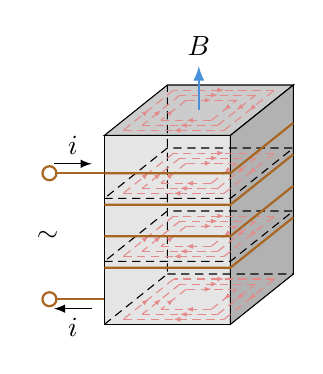
\begin{tikzpicture}[>=latex, scale=0.8]
  % \useasboundingbox(0.9,0)rectangle(5.1,5);
  \draw[fill=lightgray!40](0,0)rectangle(2,3);
  \draw[fill=gray!40](0,3)--(2,3)--(3,3.8)--(1,3.8)--cycle;
  \draw[fill=darkgray!40](2,3)--(3,3.8)--(3,0.8)--(2,0)--cycle;
  \draw[densely dashed](0,0)--(1,0.8)--(1,3.8)(1,0.8)--(3,0.8);
  \foreach \y in {0,1,2,3}
  {
    \foreach \x in {1,2,3}
    {
      \draw[red7,thin,densely dashed,postaction={decorate},decoration={markings,mark=at position 0.5 with {\arrowreversed{Latex[scale=0.5]}}}]
  (0.3*\x,0.08*\x+\y)--(2.0-0.1*\x,0.08*\x+\y);
    \draw[red7,thin,densely dashed,postaction={decorate},decoration={markings,mark=at position 0.5 with {\arrowreversed{Latex[scale=0.5]}}}]
  (2.0-0.1*\x,0.08*\x+\y)--(3-\x*0.3,0.8-0.08*\x+\y);
    \draw[red7,thin,densely dashed,postaction={decorate},decoration={markings,mark=at position 0.5 with {\arrowreversed{Latex[scale=0.5]}}}]
  (3-\x*0.3,0.8-0.08*\x+\y)--(1.0+0.1*\x,0.8-0.08*\x+\y);
    \draw[red7,thin,densely dashed,postaction={decorate},decoration={markings,mark=at position 0.5 with {\arrowreversed{Latex[scale=0.5]}}}]
  (1.0+0.1*\x,0.8-0.08*\x+\y)--(0.3*\x,0.08*\x+\y);
  }
  }
  \draw[densely dashed](0,1)--(2,1)--(3,1.8)--(1,1.8)--cycle;
  \draw[densely dashed](0,2)--(2,2)--(3,2.8)--(1,2.8)--cycle;
  \draw[thick,->,azure6](1.5,3.4)--++(0,0.7)node[above,text=black]{$B$};
  \foreach \x in {0.9,1.4,1.9,2.4}
  {
    \draw[brown5,thick](0,\x)--(2,\x)--(3,\x+0.8);
  }
  \draw[brown5,thick,o-](-1,2.4)--(0,2.4);
  \draw[brown5,thick,o-](-1,0.4)--(0,0.4);
  \node at (-0.9,1.4){$\sim$};
  \draw[->](-0.8,2.55)--(-0.2,2.55)node[midway,above]{$i$};
  \draw[<-](-0.8,0.25)--(-0.2,0.25)node[midway,below]{$i$};
\end{tikzpicture}
\end{document}